% !TEX root = main.tex
\chapter{Data Findings}
\label{Chapter:Findings}

Once the data collection method was developed and implemented, we started mining through the information collected in an attempt to answer the key questions described in chapter \ref{Chapter:Introduction} for the RTP region. We broke down those high level questions into more specific items described in section \ref{key-res-questions}. To find out about GitHub users in the RTP region, we provide answers to questions one through five. In order to see what the overall numbers look like in terms of projects developed out of the RTP area as well as their associated activity and current relevance, we answer questions six through twelve. Finally, in order to gain a better understanding of how RTP users are taking advantage of GitHub social networking features, as well as their overall popularity, we answer questions thirteen through fifteen.

We found that the easiest way to illustrate a lot of these findings was to create visual representations of the data collected. For this, we used Plot.ly, an open source framework for developing data visualizations in various languages \cite{_plotly_????}. Figure~\ref{fig:user-count-by-city-code} shows an example of the creation of a bar chart using this framework. The remainder of this chapter is broken down into specific sections dedicated to answering the key research questions. We first go into an overview of RTP users, then drill into RTP specific repositories, overall open source contribution activity and lastly look into the usage of social networking features available on GitHub.

\section{Key Research Questions}
\label{key-res-questions}
\begin{enumerate}
\item How many users does the RTP area have overall?
\item How many users does the RTP area have by type (User vs. Organization)?
\item What is the average number of repositories per user in RTP (overall)?
\item How long have local users been GitHub members? How many users have been around since GitHub started?
\item What city has the most users?
\item What is the repository count by User? 
\item What is the repository count by Organization?
\item Who has the most repositories overall in the RTP area?
\item Are users creating original repositories or forking existing repositories or collaborating more often?
\item What do the commit numbers look like for local RTP repositories?
\item How many of the RTP repositories are active (for this research, active is defined as repositories which contain changes that have been committed at some point over the last 6 months)?
\item What is the average life of a local project?
\item Are many local users being "followed"?
\item Are local repositories being starred often?
\item What are the most popular programming languages?
\end{enumerate}

\begin{figure}
\footnotesize
\begin{lstlisting}
def userCountByCity_BarChart():
    results = userCountByCity.find({"count":{"$gte" : 20}})

    x = []
    y = []

    for i in results:
        x.append(i['_id'])
        y.append(i['count'])

    plotly.offline.plot({
    "data": [
        Bar(x=x, y=y,
            marker=dict(
            color='rgb(158,202,225)',
            line=dict(
                color='rgb(8,48,107)',
                width=1.5
            ),
        ),
        opacity=0.6)
    ],
    "layout": Layout(
        title="Number Of Users By City (User Count Greater Than 20)",
        annotations=[
        dict(
            x=xi,
            y=yi,
            text=str(yi),
            xanchor='center',
            yanchor='bottom',
            showarrow=False,
        ) for xi, yi in zip(x, y)]
    )
    })
\end{lstlisting}
\normalsize
\caption{Sample Python code which pulls the total repository count per user using PyMongo and the Aggregation Framework.}
\label{fig:user-count-by-city-code}
\end{figure}

%\begin{figure}
%\begin{center}
%\resizebox{\textwidth}{!}{
%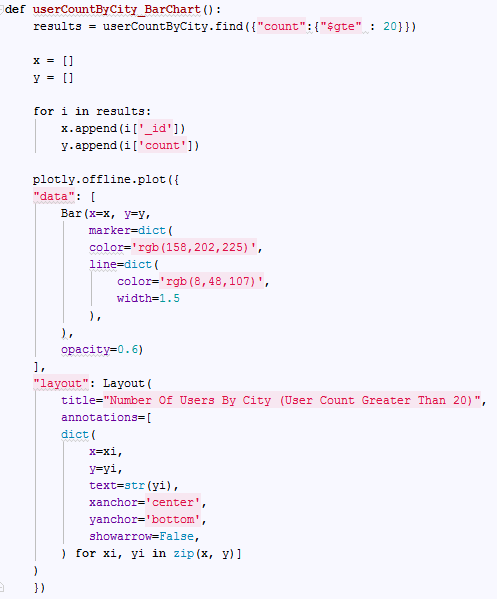
\includegraphics{Images/userCountByCity-pymongo.PNG}
%}
%\caption{Sample Python code which pulls the total repository count per user using PyMongo and the Aggregation Framework.} 
%\label{fig:user-count-by-city-code}
%\end{center}
%\end{figure}

%questions 1-5
\section{Users Overview}
In this section, we will focus on answering questions one through five from section \ref{key-res-questions}. We will find out how many users the RTP area has overall, by both User and Organization type. We will also find out how many repositories each user has on average, how long they have been members and which city in the region has the most users. The collection of RTP users was the most important dataset in this research as everything else was built upon them. As discussed in chapter \ref{Chapter:RTP}, RTP is a very prominent location for the information technology industry as a whole. We suspected we would find open source activity in the area but did not have any baselines from other locations to compare to. We managed to find 3,234 total RTP users (again, only being able to find users that had their location listed on GitHub). This means only .1\% of the RTP population (as also discussed in chapter 2, there are 3 million people living in a 60 mile radius of the park) are members of GitHub. Of these, 47 percent of them were located in Raleigh. Figure \ref{fig-userCountByCityBarChart} shows a bar chart created with Plot.ly with the number of RTP users by city. This chart only shows 8 cities as we filtered out all cities that had less than 20 users. Out of the 90 cities identified through NCLM (see \ref{fig:rtp-cities}), only 33 contained users contributing on GitHub. Raleigh, Durham and Chapel Hill had the highest number of users in the area which is understandable given these locations are home to the major research universities as well as many of the large technology companies referenced in chapter \ref{Chapter:RTP}. We also looked into the total number of RTP users by user type, finding that the majority of accounts were "User" - 2,982 with the remaining 252 being of type "Organization".

\begin{figure}
\begin{center}
\resizebox{\textwidth}{!}{
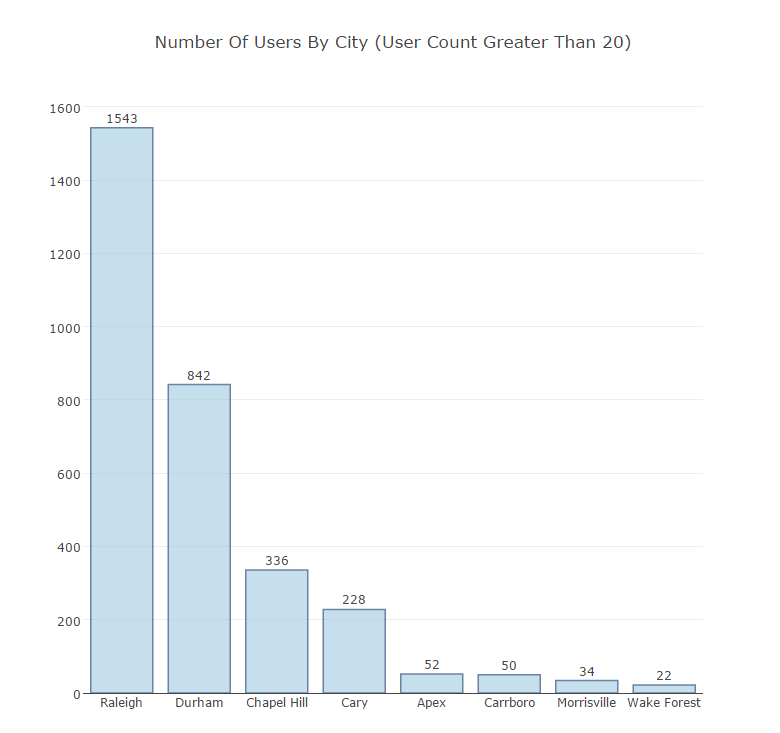
\includegraphics{Charts/userCountByCity-final.PNG}
}
\caption{This figure shows all RTP cities that have more than 20 users.} 
\label{fig-userCountByCityBarChart}
\end{center}
\end{figure}

Another metric that we were interested in gathering was how long the local RTP users had been members on GitHub. As mentioned in the previous chapter, GitHub has been around for 8 years now. We were curious to find out how many local users had created their accounts when the service went live. There ended up being around 130 users that have had their accounts for 7-8 years. Out of these accounts, 61\% (80 users) have been active (or submitted a commit) over the last 6 months. Figure \ref{fig-activeUsers} shows the script used to determine active users who have been members on GitHub for over 7 years. It was interesting to note that over half of the oldest users were still active on GitHub.

%\begin{figure}
%\label{fig-activeUsers}
%\begin{center}
%\resizebox{\textwidth}{!}{
%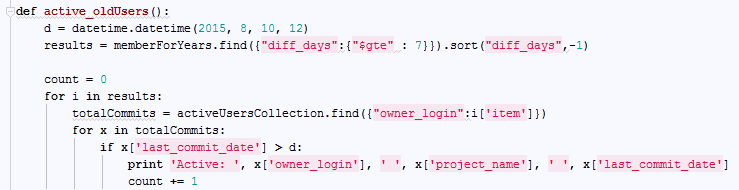
\includegraphics[width=16cm]{Images/active_legacyUsers.PNG}
%}
%\caption{This figure shows the Python script used to find RTP users that have been members on GitHub for more than 7 years and are still active today.} 
%\end{center}
%\end{figure}

\begin{figure}
\footnotesize
\begin{lstlisting}
def active_oldUsers():
  d = datetime.datetime(2015, 8, 10, 12)
  results = memberForYears.find({"diff_days":{"$gte" : 7}})
                          .sort("diff_days",-1)

  count = 0
  for i in results:
    totalCommits = activeUsersCollection.find({"owner_login":i['item']})
    for x in totalCommits:
        if x['last_commit_date'] > d:
            print 'Active: ', x['owner_login'], ' ', 
                              x['project_name'], ' ',
                              x['last_commit_date']
            count += 1
\end{lstlisting}
\caption{This figure shows the Python script used to find RTP users that have been members on GitHub for more than 7 years and are still active today.}
\label{fig-activeUsers}
\end{figure}

% questions 6-8
\section{Repositories Overview}
\label{sec:RepositoriesOverview}
In this section, we will present an overview of the RTP repositories found during the data collection phase through answering questions six through nine from section \ref{key-res-questions}. We will learn how many repositories have been created out of RTP (overall and by user type), as well as which RTP user has the most repositories. In total, we were able to find 34,825 total RTP user repositories. Of these, 31,843 were owned by a "User" type, while 2,982 were owned by an "Organization" type. There was a large amount of information available about each one of these repositories. Each repository contained an entry in a collection within our local MongoDB instance. These entries specified a number of items, including the owner details, the number of forks, whether or not the repository was a fork itself, the programming language used, the number of watchers, the create date, last updated date, as well as several API URLs that could be used to perform a number of actions on GitHub (view comment, view issues, view events, download the repository, etc.).

We calculated that RTP users have created an average of 12 repositories. The user with the most repositories had created 351, while there were a large number of users that had only created one repository. Figure \ref{fig-repoCountByUser-highest} is a chart created to show the users with the most repositories (breaking it down to users with more than 120 owned repositories). This does not necessarily mean they are active repositories and in fact could have been created and only used as a means of storage and never opened up for collaboration nor as a source code repository. The user with the most number of repositories was created as an "Organization", the account is still active today but not all 351 repositories are currently being contributed to. We will assess the activity of all repositories in section \ref{sec-ActivityOverview}. 

\begin{figure}
\resizebox{\textwidth}{!}{
\begin{bchart}[max=351]
\bcbar[text=pixbit,
 color=blue!20]{351}
\bcbar[text=jmxpearson, color=blue!20]{223}
\bcbar[text=battlemidget, color=blue!20]{193}
\bcbar[text=BanzaiMan, color=blue!20]{192}
\bcbar[text=apsaltis, color=blue!20]{155}
\bcbar[text=Rleahy22, color=blue!20]{151}
\bcbar[text=connyay, color=blue!20]{139}
\bcbar[text=vbatts, color=blue!20]{131}
\bcbar[text=pmuellr, color=blue!20]{131}
\bcbar[text=thewtex, color=blue!20]{129}
\bcbar[text=jcfr, color=blue!20]{127}
\bcbar[text=ryanfb, color=blue!20]{121}
\bcxlabel{Repository Count By User}
 \end{bchart}
}
\caption{This bar chart shows users with the most overall repositories in the RTP region.}
\label{fig-repoCountByUser-highest}
\end{figure}
             
The next piece of information gathered about overall repositories in the RTP region was the total number of original versus forked projects. We were interested in understanding if users created original projects more often than forking from already existing projects. Table \ref{fig-forked-repos} and \ref{fig-orig-repos} show the findings from these calculations. After sampling this data, we found out that around 40\% of the projects in RTP are forked and 59\% are original. This does not exclude inactive repositories. What this tells us is that while more than half of the repositories are original projects created by the RTP owner, there are still a large number of projects that have been forked from already existing projects with a possible intent to collaborate.

\begin{table}
\parbox{.45\linewidth}{
\centering
\begin{tabular}{|c|c|}
\hline
Forked Repositories & Total Users\\
\hline
15,244 & 2099\\
\hline
\end{tabular}
\caption{Total Original Repositories in RTP}
\label{fig-forked-repos}
}
\hfill
\parbox{.45\linewidth}{
\centering
\begin{tabular}{|c|c|}
\hline
Original Repositories & Total Users\\
\hline
19,745 & 2518\\
\hline
\end{tabular}
\caption{Total Forked Repositories in RTP}
\label{fig-orig-repos}
}
\end{table}

% 10-11
\section{Activity Overview}
\label{sec-ActivityOverview}
We did some investigating into how many local users were active while seeking to answer questions ten and eleven. We find out what the commit numbers look like for RTP repositories, as well as the overall activity of RTP users. As discussed previously, we defined a user as being "active" if they  have made a commit sometime over the last 6 months. We found that 2,559 unique users had made a commit over the last 6 months on GitHub which we seemed quite high. We can't necessarily say that 79\% of RTP users are active on GitHub, however, due to the fact that was discussed in chapter \ref{Chapter:Background}, when committing a change in GitHub, the author field is free text in many cases. We can see this quite clearly in the collected dataset on commits. There are unfortunately many users who lazily entered data such as their first name only (i.e. "Ben") instead of their full name, e-mail address or login name as an identifier. As part of future research, it would be useful to programatically attempt to match authors to their rightful GitHub account, similar to what the GHTorrent project does (as discussed already in section \ref{sec-GHTorrentProject}). This way we would be able to calculate a more accurate number on the total number of active users in the area.

We were able to say for certain that there are 6,756 unique RTP owned repositories that are active on GitHub, since this field cannot be free text. This means that of all the repositories owned by RTP users, 19\% of them are active. Figure \ref{fig-projCommits6mon} shows all users with more than 2,000 commits over the last 6 months. We looked a bit further into the top 10 active users (by login ID) to find out more information about them. All 10 of these users have made more than 2,000 commits to projects over the last 6 months (see Table \ref{table-top10activeusers}). As we can see, 70\% of these users are set up as Organizations on GitHub, which makes sense in that there would be more commits than "User" projects where there may be only one contributor. It was hard to identify a specific trend between these numbers. For example, these project owners either heavily utilize pull requests, or they don't. This observation could be explained by the fact that users and organizations utilize different workflows as already discussed in section \ref{sec-GitHub}.


\begin{figure}
%\resizebox{\textwidth}{!}{
\begin{bchart}[max=11.312,width=.9\textwidth]
\bcbar[text=OpenNMS, color=blue!20, value=11312]{11.312}
\bcbar[text=tee3, color=blue!20, value=3665]{3.665}
\bcbar[text=bredelings, color=blue!20, value=3145]{3.145}
\bcbar[text=duke-libraries, color=blue!20, value=2809]{2.809}
\bcbar[text=mautic, color=blue!20, value=2788]{2.788}
\bcbar[text=caktus, color=blue!20, value=2738]{2.738}
\bcbar[text=automatak, color=blue!20, value=2684]{2.684}
\bcbar[text=waldenraines, color=blue!20, value=2407]{2.407}
\bcbar[text=pencilblue, color=blue!20, value=2357]{2.357}
\bcbar[text=UNC-Libraries, color=blue!20, value=2234]{2.234}
\bcbar[text=jhinkey, color=blue!20, value=2149]{2.149}
\bcbar[text=deads2k, color=blue!20, value=2077]{2.077}
\bcxlabel{Total Commits per User}
 \end{bchart}
%}
\caption{This figure shows all users with more than 1000 commits over the last 6 months.}
\label{fig-projCommits6mon}
\end{figure}


\begin{table}
\centering
\resizebox{\textwidth}{!}{
\begin{tabular}{|c|c|c|c|c|c|c|}
\hline
User ID & User Type & Member Since & City & \# Projects & \# Pull Reqs & \# Stargazers \\
\hline
OpenNMS & Organization & Dec-12 & Pittsboro & 66 & 864 & 254 \\
\hline
tee3 & User & Mar-10 & Raleigh & 18 & 2 & 5 \\
\hline
bredelings & User & Oct-09 & Durham & 8 & 2 & 15 \\
\hline
duke-libraries & Organization & Oct-12 & Durham & 52 & 2310 & 40 \\
\hline
mautic & Organization & Aug-13 & Raleigh & 14 & 718 & 479 \\
\hline
caktus & Organization & Apr-10 & Durham & 89 & 1602 & 856 \\
\hline
automatak & Organization & Jan-13 & Raleigh & 10 & 42 & 81\\
\hline
waldenraines & User & Apr-13 & Raleigh & 17 & 0 & 0 \\ 
\hline
pencilblue & Organization & Feb-14 & Raleigh & 15 & 751 & 1257 \\
\hline
UNC-Libraries & Organization & Jan-11 & Chapel Hill & 28 & 766 & 157 \\
\hline
\end{tabular}
}
\caption{More information on the top 10 active RTP users (have pushed commits in the last 6 months). This chart shows their total number of projects, pull requests and stargazers. }
\label{table-top10activeusers}
\end{table} 

%12-14
\section{Popularity Overview}
\label{sec-PopularityOverview}
Finally, after reviewing metrics on RTP users, their repositories and overall activity on GitHub, we decided to take a look into the data to find out how "popular" our local users and projects were. In this section, we will discuss questions twelve through fifteen. We will seek to find out if many RTP users are being "followed" or "starred". We will also find out what the most popular programming language is. As mentioned in chapter \ref{Chapter:Background}, GitHub gives us an easy way to do this with their built in social media features such as "stargazing". We were able to dig into the collected data to find out that some of our users are actually somewhat popular. 1,253 users (39\%) contain at least one follower. We have 2 local users that have more than 10,000 followers. Figure \ref{fig-stargazersByUser} gives us a view of the number of stargazers that each user has (where the total number of followers is greater than 1000). The RTP user with the most stargazers is an author of a book on PHP, who lives and works in Chapel Hill.

\begin{figure}
%\resizebox{\textwidth}{!}{
\begin{bchart}[max=125.71,width=.9\textwidth]
\bcbar[text=codeguy, color=blue!20, value=12571]{125.71}
\bcbar[text=fogleman, color=blue!20, value=11682]{120.82}
\bcbar[text=jlong, color=blue!20, value=7856]{80.56}
\bcbar[text=alebcay, color=blue!20, value=6249]{70.49}
\bcbar[text=twotoasters, color=blue!20, value=3798]{60.98}
\bcbar[text=cognitect, color=blue!20, value=2586]{55.86}
\bcbar[text=smashingboxes, color=blue!20, value=2428]{50.28}
\bcbar[text=jaymedavis, color=blue!20, value=1564]{45.64}
\bcbar[text=clojure-cookbook, color=blue!20, value=1554]{40.54}
\bcbar[text=alandipert, color=blue!20, value=1553]{39.53}
\bcbar[text=mapier, color=blue!20, value=1304]{35.04}
\bcbar[text=pencilblue, color=blue!20, value=1257]{33.57}
\bcbar[text=kconner, color=blue!20, value=1204]{31.04}
\bcbar[text=stuarthalloway, color=blue!20, value=1187]{29.87}
\bcbar[text=bwsewell, color=blue!20, value=1145]{27.45}
\bcbar[text=yfactorial, color=blue!20, value=1073]{24.073}
\bcxlabel{Total Stargazers per User}
 \end{bchart}
%}
\caption{This figure shows the number of followers that each user has (where the count of followers is greater than 1000).}
\label{fig-stargazersByUser}
\end{figure}

Another metric we collected was the overall programming language popularity in this region. We aggregated the repository collections and counted the number of occurrences for each language, ignoring any projects that did not have the programming language listed (8,459 or 24\% did not have one listed). Figure \ref{fig-progLangPopularity} shows the number of projects that use each language in a bar chart where usage count is greater than 1,000, with JavaScript leading the way. We note that this information is what comes back from GitHub, it is important to remember that many projects will likely have more than one associated programming language.

\begin{figure}
%\resizebox{\textwidth}{!}{
\begin{bchart}[max=5.467,width=.9\textwidth]
\bcbar[text=JavaScript, color=blue!20, value=5467]{5.467}
\bcbar[text=Ruby, color=blue!20, value=4527]{4.527}
\bcbar[text=Python, color=blue!20, value=3457]{3.457}
\bcbar[text=Java, color=blue!20, value=2062]{2.062}
\bcbar[text=CSS, color=blue!20, value=1349]{1.349}
\bcbar[text=PHP, color=blue!20, value=1255]{1.255}
\bcbar[text=Shell, color=blue!20, value=1069]{1.069}
\bcxlabel{Top GitHub Programming Languages in RTP}
 \end{bchart}
%}
\caption{This figure shows the most popular programming languages in the RTP region, where the usage count is greater than 1000.}
\label{fig-progLangPopularity}
\end{figure}


%15
\section{Average Life of a RTP Project}
\label{sec-lifeOfAProj}
One of the additional data points that we decided to collect was what the average life of a GitHub project owned by a user in RTP looked like (question fifteen). We found out that the oldest RTP repository was created less than a month after GitHub was founded, "depth-charge". Figure \ref{fig-mongoqueryOldestRTPRepo} shows the query used to find this information in our local MongoDB database. This particular repository was created 8 years ago and hasn't been updated since.

\begin{figure}
\label{fig-mongoqueryOldestRTPRepo}
\begin{lstlisting}
> db.githubRTPUsersRepos
	.find({},
    	{"owner.login":1,"created_at":"1","name":1})
    .sort({"created_at":1})
    .limit(1)
> { 
	"_id" : ObjectId("52bedd67bd3543677400823a"), 
	"owner" : { "login" : "bscofield" }, 
    	"name" : "depth-charge", 
    	"created_at" : ISODate("2008-02-27T12:42:10Z") 
  }
\end{lstlisting}
\caption{Finding the oldest RTP repository from MongoDB's shell  (query and result).}
\end{figure}

Finally, we also found that the average life of a RTP project is 102 days. This was calculated by subtracting the created date from the last commit date and then averaging the entire gathered list. We found that the shortest project was 1 day and that there are plenty of projects that are still ongoing and active.

\section{Threats to Validity}
Due to the quality of data that we were able to retrieve for this project, there are several threats to validity that must be mentioned. As already discussed, it is important to remember that the location field in GitHub is not required, hence there is likely a large population of users that are left out of our research because they haven't given a location or have possibly given an inaccurate one. This was a limitation with our research due to the fact that we were heavily interested in querying for users that lived in such a specific location. Additionally, it was difficult for us to find out the exact number of commits per user. This is because users are able to enter free text into the authors field when committing a change in the GitHub shell (command line). This impacted the results from the mining for overall activity in the RTP region. We looked into pulling data from other sources to supplement the information from GitHub. An example source being LinkedIn, which was unsuccessful due to restrictions with the licensing of their REST API.
